\chapter{Uživatelské rozhraní}
\label{chap:ui}

Uživatelské rozhraní (anglicky \textit{User Interface}, zkráceně UI) je vrstva systému, která zajišťuje komunikaci mezi uživatelem a aplikací nebo zařízením \cite{smashing-ui}. Cílem každého uživatelského rozhraní je prezentace informací a poskytnutí nástrojů pro manipulaci se systémem. Takové systémy bývají často zaměřeny na různorodé skupiny lidí odlišných národností a zaměření, jejich cíl je však většinou spojuje -- usilují o rychlou, efektivní a intuitivní práci. Úkolem kvalitního uživatelského rozhraní je cílové skupině lidí tyto vlastnosti poskytovat.

Je důležité poznamenat, co vlastně návrh uživatelského rozhraní zahrnuje -- nejedná se pouze o rozložení jednotlivých prvků a vizuální stránku vytvářeného systému. Důležitým prvkem je také zvolení správných prvků a nástrojů se kterými uživatelé manipulují. I v případě, že uživatel pracuje se systémem poprvé musí určité elementy působit povědomě.

\section{Grafické uživatelské rozhraní}
\label{sec:gui}

Grafické uživatelské rozhraní (anglicky \textit{Graphical User Interface}, dále jen GUI) je typ uživatelského rozhraní, které umožňuje jednoduchou práci s elektronickým zařízením (popř. aplikací). Tato vlastnost je zajištěna použitím vhodných prvků, které poskytují intuitivní nástroje se daným typem systému (např. použití vhodných ikonek, tlačítek, oken atd.).

Na vývoj grafických uživatelských rozhraní má vliv mnoho aspektů mezi něž patří mimo jiné i způsob interakce člověka s počítačem. Už na začátku osmdesátých let se začali objevovat první polohovací zařízení, díky kterým se postupně eliminovaly nedostatky textových rozhraní -- především jejich nemožná integrovatelnost mezi běžné uživatele. Tím vznikla základní podoba WIMP konceptu (\textit{Windows, Icons, Menus, Pointer}), která představuje elementární rysy dnešních GUI.

\begin{figure}[htbp]
    \centering
    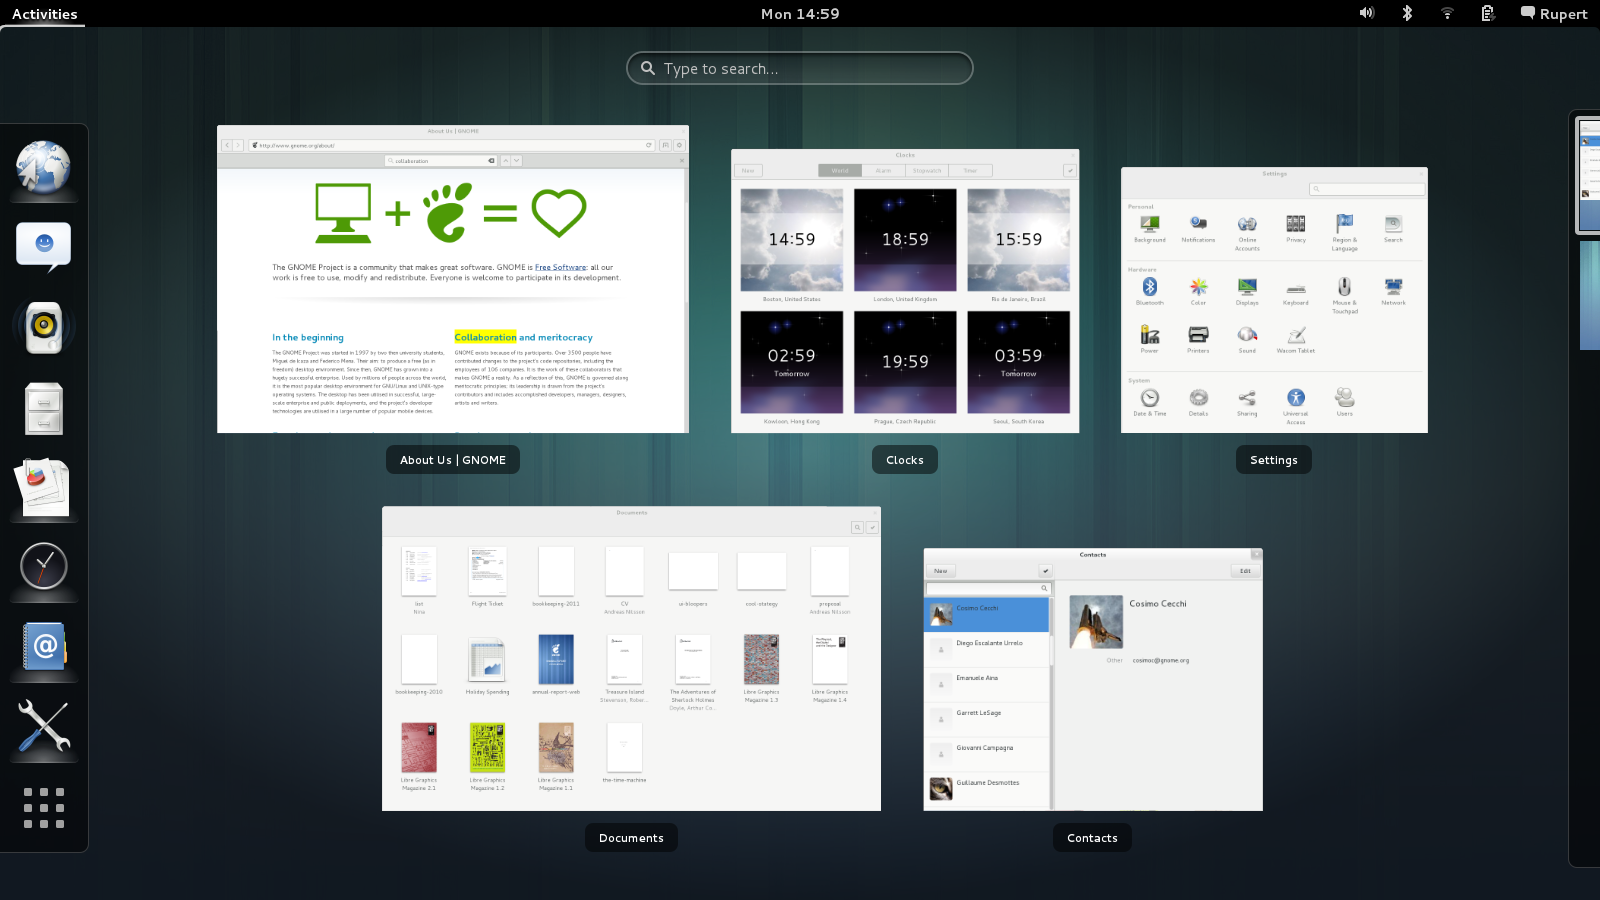
\includegraphics[width=\textwidth]{images/gui-example.png}
    \caption{Příklad GUI (zdroj: \url{https://live.gnome.org/}).}
\end{figure}

Považuji za vhodné poznamenat, že pojem \textit{grafické uživatelské rozhraní} bývá často používán výhradně pro označení rozhraní, které umožňují uživatelům komunikovat s elektronickými zařízeními (integrovaných např. v operačním systému). Tato definice je však nepřesná, neboť neoznačuje systémy, které operují jako tzv. tenký klient. Tenký klient je druh systému, jehož funkčnost je závislá na jiném zařízení (serveru). Takové systému slouží především pro projekci informací uživateli, zatímco zpracování a ukládání dat provádí server. Příkladem aplikace, která pracuje na tomto typu architektury je například Internetový prohlížeč.

\section{Webové uživatelské rozhraní}
\label{sec:wui}

Webové uživatelské rozhraní (anglicky \textit{Web-based User Interface}, dále jen WUI) je typ grafického uživatelského rozhraní, které je součástí webových aplikací. Webová aplikace je typ programu, jehož funkce a nástroje jsou přístupné přes HTTP protokol\footnote{\textit{HyperText Transfer Protocol} je internetový protokol, který definuje způsob jakým jsou data na webu formátovány a přenášeny -- původně byl tento druh komunikace zajištěn výměnou převážně hypertextových dokumentů, aktuální verze však podporuje i další formáty (XML, JSON, HTML, PDF atd.).}. Interakce mezi uživatelem a programem je pak zajištěna webovým prohlížečem.

\begin{figure}[htbp]
    \centering
    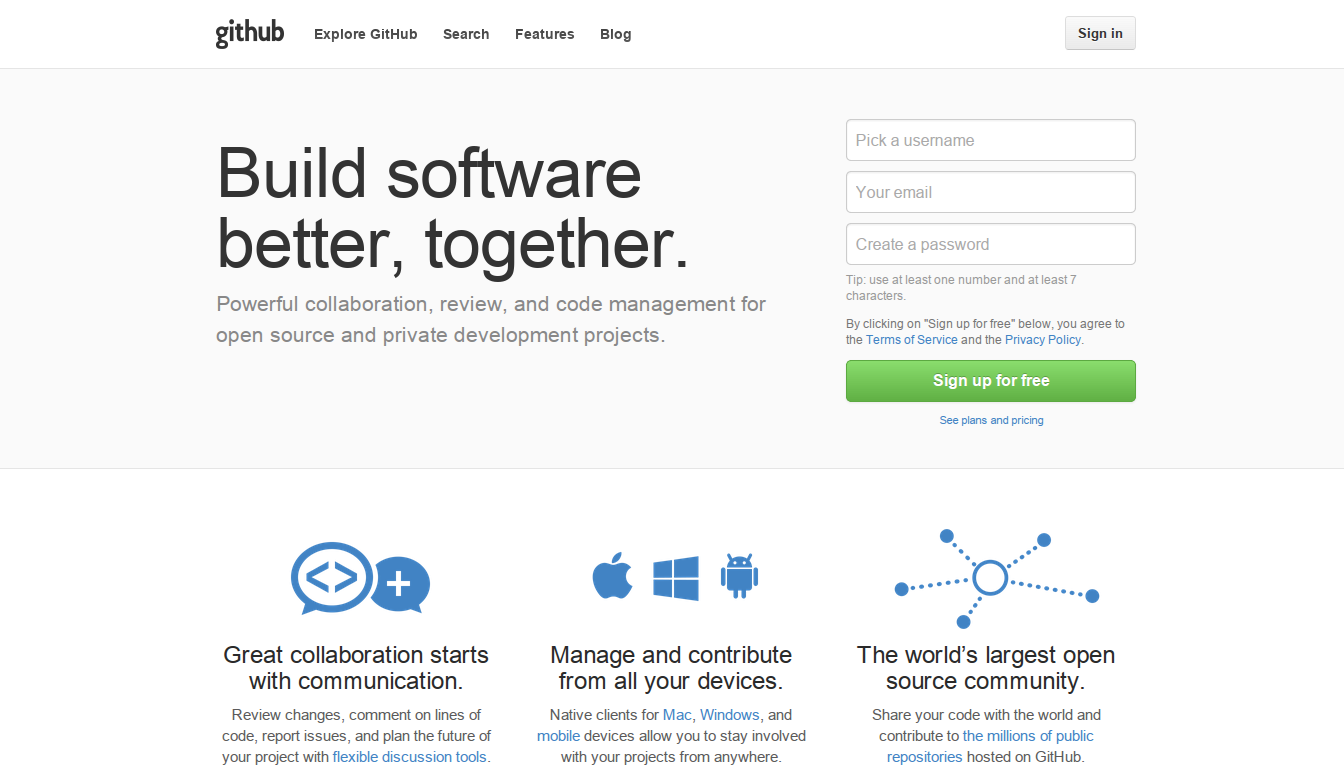
\includegraphics[width=\textwidth]{images/wui-example.png}
    \caption{Příklad WUI (zdroj: \url{https://github.com/}).}
\end{figure}

Mezi hlavní výhody webových aplikací patří relativně jednoduchá udržovatelnost a flexibilita. Tyto vlastnosti jsou dány povahou klient--server modelu. Jedná se o síťovou architekturu, která rozlišuje klienta (uživatele) a server (aplikaci). Klient--server model umožňuje vývojářům udržovat pouze jednu verzi aplikace, která je multiplatformní a často daleko bezpečnější a spolehlivější. Nevýhodou je nižší dostupnost a vyšší odezva, která je dána kvalitou síťového (Internetového) připojení.

\section{Proces tvorby uživatelského rozhraní}
\label{sec:process}

\begin{quote}
\uv{Proces tvorby uživatelského rozhraní je zdokumentovaný postup, který je nutné absolvovat pro dokončení typického uživatelského rozhraní.}
\end{quote}

\noindent
Vývoj každého systému prochází několika fázemi, které se většinou překrývají převážně z důvodu spolupráce vývojářů, designérů a analytiků. Tyto fáze lze rozdělit na čtyři části.

\begin{enumerate}[leftmargin=1cm]
    \item \textbf{Plánování}\\
          Představuje analýzu požadavků klienta a cílové skupiny uživatelů. Dále je v tomto stádiu stanoven výběr programovacích jazyků, knihoven a dalších nástrojů, které budou použity v implementaci.

    \item \textbf{Design}\\
          Informace shromážděné z předchozího stádia jsou sepsány a analyzovány. Návrh doprovází vývoj struktury a vizuální podoby aplikace, přičemž je obvykle rozdělen do tří částí -- tvorba drátěného modelu, grafického návrhu a kódování šablon. Tyto kroky mají za úkol podrobněji specifikovat požadavky klienta a odhalit nejasnosti v zadání ideálně již na počátku vývoje. Návrh probíhá převážně paralelně s vývojem.

    \item \textbf{Vývoj}\\
          V této fázi jsou požadované funkce systému implementovány za použití ustanovených technologií a knihoven. Vývoj také zahrnuje verifikaci požadavků, integraci grafických návrhů do systému a testování systému včetně použitelnosti.

    \item \textbf{Spuštění}\\
           Jedná se o poslední fázi, která prochází nejdelším cyklem. Systém je nasazen na produkci, což umožňuje hlubší testování koncovými uživateli. Zároveň jsou prováděny poslední kroky pro vypilování použitelnosti a tvorbu dokumentace.

\end{enumerate}

Produkce uživatelského rozhraní je provázána se všemi těmito fázemi a zahrnuje několik aktivit, které vyžadují práci s různými nástroji a technologiemi. Tyto aktivity vyžadují rozdílné znalosti a jsou často rozděleny mezi specificky zaměřené designéry.

\subsection{Tvorba drátěného modelu}
\label{sec:wireframing}

\begin{figure}[htbp]
    \centering
    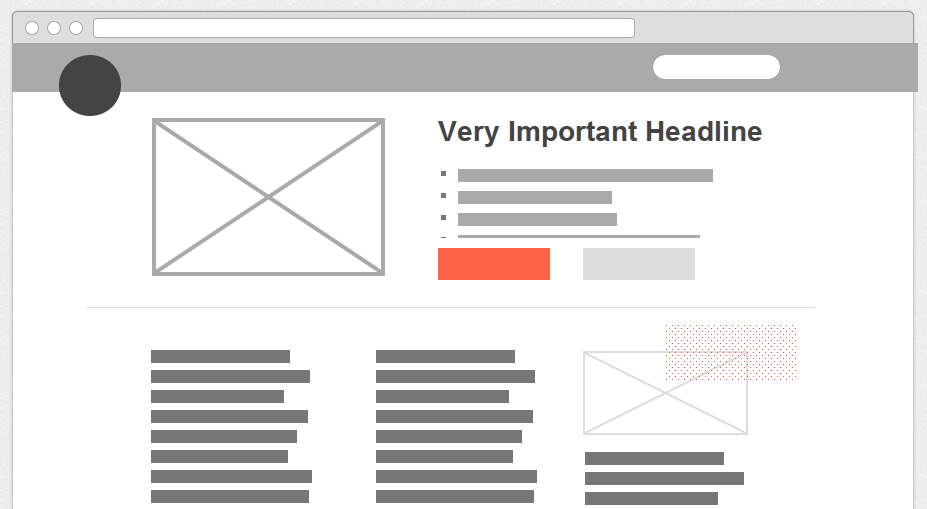
\includegraphics[width=\textwidth]{images/wireframe-example.png}
    \caption{Příklad drátěného modelu (zdroj: \url{http://wireframe.cc/}).}
\end{figure}

Webový drátěný model (anglicky \textit{wireframe}) je zjednodušená kresba, která reprezentuje rozmístění prvků a komponent webové stránky; prezentuje strukturální úroveň. Tvorba drátěného modelu zaujímá místo již na začátku životního cyklu projektu a slouží pro zachycení základní struktury stránky. Úkol drátěného modelu je poskytnout vizuální porozumění stránky již na počátku tvorby uživatelského rozhraní.

Přední výhodou drátěných modelů je jednoduchá přizpůsobitelnost potřebám klienta a jasně definovaná kostra, která zajišťuje sebedůvěru designéra. V pozdějších fázích projektu by se neměl drátěný model nijak zásadně měnit a měl by odpovídat grafickému návrhu.

\subsection{Tvorba grafického návrhu}
\label{sec:designing}

Grafický návrh poskytuje vizuální podobu webové aplikace; reprezentuje aplikaci v podobě, ve které bude prezentována uživateli. Tato fáze zahrnuje výběr grafických a typografických prvků. Mezi grafické prvky obyčejně patří kombinace barev, obrázků, tvar tlačítek apod. Typografické prvky zahrnují především organizaci písma -- volbu řezů a rodin písma pro odlišení jednotlivých částí webové stránky. Dále zahrnují velikosti odstavců, použití odrážek, řádkování atd.

\subsection{Kódování}
\label{sec:coding}

V tomto stádiu přichází na řadu rozřezání a kódování grafického návrhu. Kódování probíhá formou HTML (\textit{HyperText Markup Language}) a CSS (\textit{Cascading Style Sheets}), což jsou technologie určené primárně pro prezentaci dokumentů na webu. Kód by měl být psán s ohledem na W3C standard\footnote{W3C (\textit{World Wide Web Consortium}) je mezinárodní konsorcium, které se stará o vývoj webových standardů.}, zároveň je doporučeno dodržovat osvědčené postupy\footnote{Doporučené postupy při vývoji HTML dokumentů jsou vystaveny například společností Creative Technology (\url{http://isobar-idev.github.io/code-standards/})} pro zvýšení čitelnosti a podpory všech populárních prohlížečů.
